\documentclass{beamer}
\usepackage{graphicx}
\usepackage{caption}
\usepackage{subcaption}
\graphicspath{ {./figures/} }
\title{Tomografie a Radonova transformace}
\author{Dominika Hájková, Matyáš Fuksa, Ondřej Kureš}
\institute{Skupina W}
\date{2021}

\begin{document}

\frame{\titlepage}

\begin{frame}
\frametitle{1. stránka}
Ano, zde je 1. stránka této prezentace. Něco pěkného sem pak vložíme.
\end{frame}
\begin{frame}
\frametitle{2. stránka}
Překvapivě, zde je 2. stránka této prezentace. Pro zachování rovnováhy, na tuto stránku vložíme něco nepěkného.
\end{frame}
\begin{frame}
\frametitle{3. stránka}
Pro ty, co to nečekali, zde je 3. stránka této prezentace. Když už jsme vše uvedli do rovnováhy, tak sem nevložíme nic.
\end{frame}

\begin{frame}
\frametitle{Co snědla Vítkova dcerka?}

\begin{figure}
\centering
\begin{subfigure}{.5\textwidth}
  \centering
  
\includegraphics[width=.8\linewidth]{secret-radon.pdf}
  \label{fig:sub1}
\end{subfigure}%
\begin{subfigure}{.5\textwidth}
  \centering
  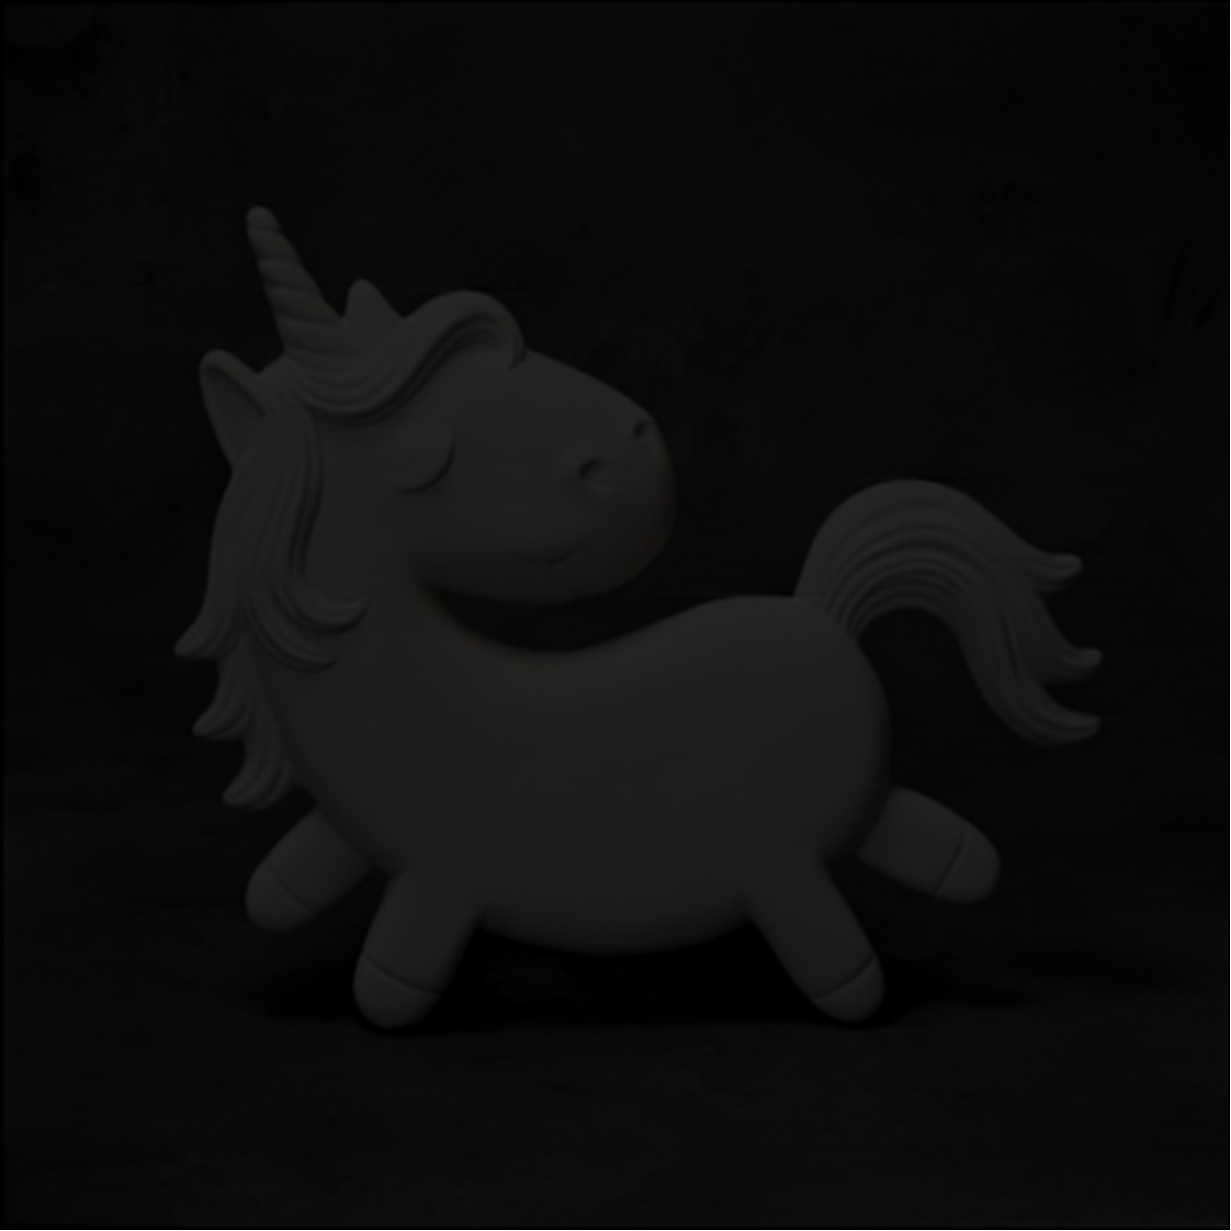
\includegraphics[width=.8\linewidth]{unicorn.pdf}
  \label{fig:sub2}
\end{subfigure}
\caption{Skrytý obrázek a odhalený obrázek}
\label{fig:test}
\end{figure}

\end{frame}
\end{document}